\documentclass{sigchi-ext}
% Please be sure that you have the dependencies (i.e., additional
% LaTeX packages) to compile this example.
\usepackage[T1]{fontenc}
\usepackage{textcomp}
\usepackage[scaled=.92]{helvet} % for proper fonts
\usepackage{graphicx} % for EPS use the graphics package instead
\usepackage{balance}  % for useful for balancing the last columns
\usepackage{booktabs} % for pretty table rules
\usepackage{ccicons}  % for Creative Commons citation icons
\usepackage{ragged2e} % for tighter hyphenation

% \usepackage{marginnote} \usepackage[shortlabels]{enumitem}
% \usepackage{paralist}

% EXAMPLE BEGIN -- HOW TO OVERRIDE THE DEFAULT COPYRIGHT STRIP --
 \copyrightinfo{Permission to make digital or hard copies of all or
 part of this work for personal or classroom use is granted without
 fee provided that copies are not made or distributed for profit or
 commercial advantage and that copies bear this notice and the full
 citation on the first page. Copyrights for components of this work
 owned by others than ACM must be honored. Abstracting with credit is
 permitted. To copy otherwise, or republish, to post on servers or to
 redistribute to lists, requires prior specific permission and/or a
 fee. Request permissions from permissions@acm.org.\\
 {\emph{CHI'14}}, April 26--May 1, 2014, Toronto, Canada. \\
 Copyright \copyright~2014 ACM ISBN/14/04...\$15.00. \\
 DOI string from ACM form confirmation}
% EXAMPLE END

\title{Study Social: Forming Study Groups Online Through Social Media}

\numberofauthors{4}
% Notice how author names are alternately typesetted to appear ordered
% in 2-column format; i.e., the first 4 autors on the first column and
% the other 4 auhors on the second column. Actually, it's up to you to
% strictly adhere to this author notation.
\author{%
  \alignauthor{%
    \textbf{Kai Anderson}\\
    \affaddr{Utah State University} \\
    \affaddr{Logan, UT 84321, USA} \\
    \affaddr{kai.thomas.anderson@gmail.com} }\alignauthor{%
    \textbf{Erik Falor}\\
    \affaddr{Utah State University} \\
    \affaddr{Logan, UT 84321, USA} \\
    \email{ewfalor@gmail.com} } \vfil \alignauthor{%
    \textbf{Maur\'{i}el Ramirez}\\
    \affaddr{Utah State University} \\
    \affaddr{Logan, UT 84321, USA} \\
    \email{mauriel.ramirez@gmail.com} }\alignauthor{%
    \textbf{Alan Williams}\\
    \affaddr{Utah State University} \\
    \affaddr{Logan, UT 84321, USA} \\
    \email{alan.williams@aggiemail.usu.edu} } \vfil  }




% Paper metadata (use plain text, for PDF inclusion and later
% re-using, if desired)
\def\plaintitle{Study Social: Forming Study Groups Online Through Social Media} \def\plainauthor{Kai Anderson, Erik Falor, Maur\'{i}el Ramirez, Alan Williams}
\def\plainkeywords{
	Social Media; Study Groups; Study Habits; Dating Service}
\def\plaingeneralterms{Documentation, Standardization}

%% Set up our PDF with metadata
\hypersetup{%
  pdftitle={\plaintitle}, pdfauthor={\plainauthor},
  pdfkeywords={\plainkeywords}, }

% \reversemarginpar%

\begin{document}

\maketitle

% Uncomment to disable hyphenation (not recommended)
% https://twitter.com/anjirokhan/status/546046683331973120
\RaggedRight{} 

% Do not change the page size or page settings.
\begin{abstract}
	College students seeking a compatible study group or tutor face a challenge
	as difficult as finding a date. The same tools and techniques used to find
	a date online can be applied to studying.
	Abstracts should be about 150 words. Required.
\end{abstract}

\keywords{\plainkeywords}

\category{H.1.2}{User/Machine Systems}{Human factors, Software psychology}
\category{H.5.2}{User Interfaces}{Graphical user interfaces, prototyping, User-centered design, Interaction styles}
\category{H.5.3}{Groups and Organization Interfaces}{Asynchronous interaction, Collaborative computing, Computer-supported cooperative work, Organizational design, Web-based interaction}

\section{Introduction}
KAI ANDERSON KAI ANDERSON KAI ANDERSON KAI ANDERSON KAI ANDERSON KAI ANDERSON 
Lorem ipsum dolor sit amet, consectetuer adipiscing elit. Aenean
commodo ligula eget dolor. Aenean massa. Cum sociis natoque penatibus
et magnis dis parturient montes, nascetur ridiculus mus. Donec quam
felis, ultricies nec, pellentesque eu, pretium quis, sem. Nulla
consequat massa quis enim. Donec pede justo, fringilla vel, aliquet

\marginpar{%
  \vspace{-45pt} \fbox{%
    \begin{minipage}{0.925\marginparwidth}
      \textbf{Good Utilization of the Side Bar} \\
      \vspace{1pc} \textbf{Preparation:} Do not change the margin
      dimensions and do not flow the margin text to the
      next page. \\
      \vspace{1pc} \textbf{Materials:} The margin box must not intrude
      or overflow into the header or the footer, or the gutter space
      between the margin paragraph and the main left column. The text
      in this text box should remain the same size as the body
      text. Use the \texttt{{\textbackslash}vspace{}} command to set
      the margin
      note's position. \\
      \vspace{1pc} \textbf{Images \& Figures:} Practically anything
      can be put in the margin if it fits. Use the
      \texttt{{\textbackslash}marginparwidth} constant to set the
      width of the figure, table, minipage, or whatever you are trying
      to fit in this skinny space.
    \end{minipage}}\label{sec:sidebar} }



\section{Literature Review}
KAI ANDERSON KAI ANDERSON KAI ANDERSON KAI ANDERSON KAI ANDERSON
``An expert neural network system for dynamic job shop scheduling''~\cite{sim1994expert}
nec, vulputate eget, arcu. In enim justo, rhoncus ut, imperdiet a,
``Too much information''~\cite{christensen2006too}
venenatis vitae, justo. Nullam dictum felis eu pede mollis pretium.
``Real-time recommendations for user-item streams''~\cite{lommatzsch2015real}
Integer tincidunt. Cras dapibus. Vivamus elementum semper nisi. Aenean
``Love me Tinder: Untangling emerging adults' motivations for using the dating application Tinder''~\cite{sumter2017love}
vulputate eleifend tellus. Aenean leo ligula, porttitor eu, consequat
``Interaction-based collaborative filtering methods for recommendation in online dating''~\cite{krzywicki2010interaction}
vitae, eleifend ac, enim. Aliquam lorem ante, dapibus in, viverra quis,
``Binder: the Tinder for Studying''~\cite{binder}



\section{Investigative Research}
ALAN WILLIAMS ALAN WILLIAMS ALAN WILLIAMS ALAN WILLIAMS ALAN WILLIAMS 
feugiat a, tellus. Phasellus viverra nulla ut metus varius laoreet.
Quisque rutrum. Aenean imperdiet. Etiam ultricies nisi vel augue.
Curabitur ullamcorper ultricies nisi. Nam eget dui.
Etiam rhoncus. Maecenas tempus, tellus eget condimentum rhoncus, sem
quam semper libero, sit amet adipiscing sem neque sed ipsum. Nam quam

\begin{figure}
  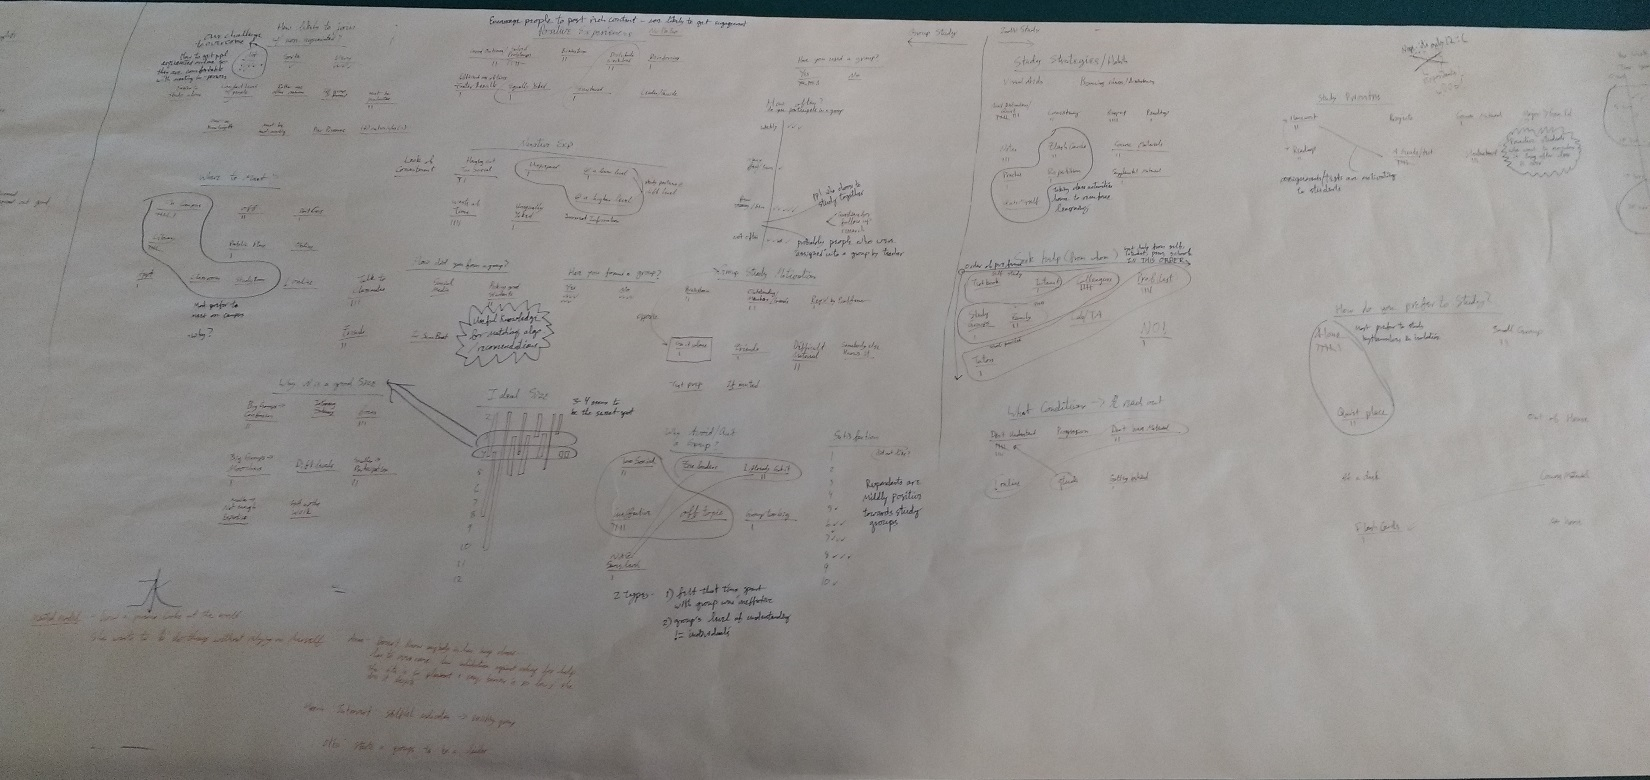
\includegraphics[width=0.9\columnwidth]{figures/affinity_diagram.jpg}
  \caption{Affinity diagram}~\label{fig:sample}
\end{figure}

\begin{marginfigure}[-15pc]
  \begin{minipage}{\marginparwidth}
    \centering
    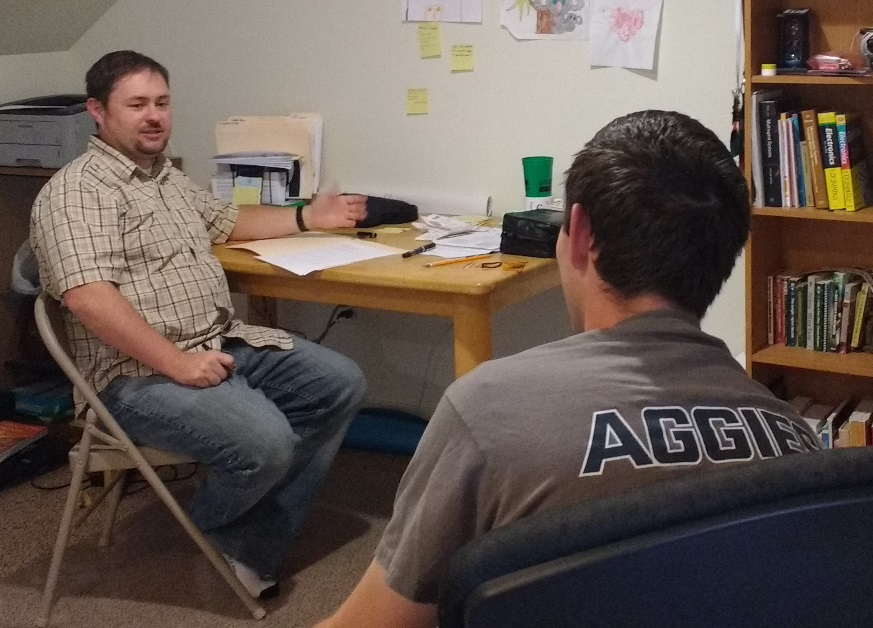
\includegraphics[width=0.9\marginparwidth]{figures/user_study.jpg}
    \caption{A user study was undertaken as one-on-one interviews with 12 subjects.}~\label{fig:marginfig}
  \end{minipage}
\end{marginfigure}



\section{Personas and Scenarios}
ALAN WILLIAMS ALAN WILLIAMS ALAN WILLIAMS ALAN WILLIAMS ALAN WILLIAMS 
\textbf{TODO:}
\textit{Let's find some photographs to go a long with each of our personas.
We can throw that over into the gutter}
quam semper libero, sit amet adipiscing sem neque sed ipsum. Nam quam
nunc, blandit vel, luctus pulvinar, hendrerit id, lorem. Maecenas nec
odio et ante tincidunt tempus. Donec vitae sapien ut libero venenatis
faucibus. Nullam quis ante. Etiam sit amet orci eget eros faucibus
tincidunt. Duis leo. Sed fringilla mauris sit amet nibh. Donec sodales
sagittis magna. Sed consequat, leo eget bibendum sodales, augue velit

\marginpar{\vspace{5pc}So long as you don't type outside the right
  margin or bleed into the gutter, it's okay to put annotations over
  here on the left, too. You'll have to manually align the margin
  paragraphs to your \LaTeX\ floats using the
  \texttt{{\textbackslash}vspace{}} command.}



\section{Prototyping}
We began the design process on paper by sketching several concepts for the
pages comprising the application. After settling on a concept we created a
digital prototype using the JustInMind Prototyping tool~\cite{justinmind}. This
software program allowed our team to create a hi-fidelity interactive prototype
with the ease of making a drawing. 

\textbf{TODO:} \textit{Heuristic evaluation: did we do one of these?}
Having an interactive prototype made our cognitave walkthrough easy because it was
natural to give our subjects a webpage to use. They were already familiar with the
concept of a webpage and knew how to use one, so we didn't weird them out by giving
them a stack of papers with the instruction to ``use your imagination.''

The cognative walkthrough revealed some weaknesses in our design which we had
theretofore been blind to. Our navigation scheme was insufficient and
inconsistent, leaving users lost and confused. Users were unsure as to whether
the data they had painstakingly input had been saved, and searched in vain for
a save button.


\begin{marginfigure}[-55pc]
	\begin{minipage}{\marginparwidth}
		\centering
		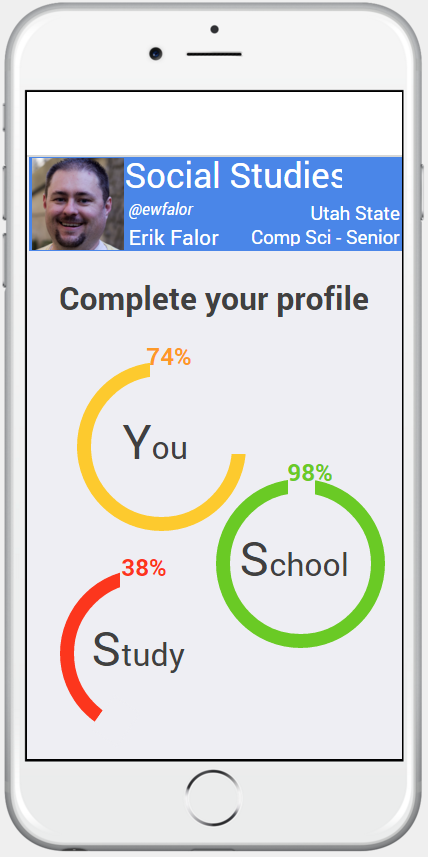
\includegraphics[width=0.9\columnwidth]{figures/prototype1.png}
		\caption{Profile landing page of the initial prototype}~\label{fig:prototype}
	\end{minipage}
\end{marginfigure}



\section{Usability Testing}
ERIK FALOR ERIK FALOR ERIK FALOR ERIK FALOR ERIK FALOR ERIK FALOR ERIK FALOR
luctus et ultrices posuere cubilia Curae; Sed aliquam, nisi quis
porttitor congue, elit erat euismod orci, ac placerat dolor lectus quis
orci. Phasellus consectetuer vestibulum elit. Aenean tellus metus,
bibendum sed, posuere ac, mattis non, nunc. Vestibulum fringilla pede
sit amet augue. In turpis. Pellentesque posuere. Praesent turpis.



\section{Conclusions}
KAI ANDERSON KAI ANDERSON KAI ANDERSON KAI ANDERSON KAI ANDERSON
luctus et ultrices posuere cubilia Curae; In ac dui quis mi
consectetuer lacinia.
Nam pretium turpis et arcu. Duis arcu tortor, suscipit eget, imperdiet
nec, imperdiet iaculis, ipsum. Sed aliquam ultrices mauris. Integer
ante arcu, accumsan a, consectetuer eget, posuere ut, mauris. Praesent



\section{Acknowledgements}
We are grateful to all of the participants who volunteered through interviews,
cognative walkthroughs, usability tests and in other activities. Their input
was invaluable and really helped this project take shape.
We owe a debt of gratitude to our helpful and enthusiastic mentor and advisor,
Dr. Amanda Hughes. We could never have created such a successful prototype
without her brilliant insight and helpful advice.
Some of the references cited in this paper are included for illustrative purposes only.



\balance{} 

% \bibliographystyle{ACM-Reference-Format-Journals}
\bibliographystyle{SIGCHI-Reference-Format}
% \bibliographystyle{acm}
\bibliography{Team-FTW-Report}

\end{document}

%%% Local Variables:
%%% mode: latex
%%% TeX-master: t
%%% End:
